% !TEX root = Master.tex

Copulas which can be derived from known multivariate distributions like for example the \textit{Multivariate Normal (or Gaussian) Distribution} or the \textit{Multivariate Student's t-Distribution} are called \textit{implicit copulas}. \textit{Elliptical copulas} are implicit copulas which arise via Sklar's theorem from elliptical distributions like the mentioned examples.\\

\textbf{Gaussian Copula}\\
W.l.o.g., for a random vector $\bm{X} \sim {\mathcal{N}_{d}(\bm{0}, \mathbf{P})} $ and \textit{correlation matrix} $\bm{P}$,
the \textit{Gaussian copula (family)} is given by
\begin{equation}
C_{\mathbf{P}}^{G a}(\mathbf{u})=\Phi_{\mathbf{P}}\left(\Phi^{-1}\left(u_{1}\right), \ldots, \Phi^{-1}\left(u_{d}\right)\right),
\end{equation}
where $\Phi$ is the \ac{CDF} of $\mathcal{N}(0, \sigma^{2})$ and 
$\Phi_{\bm{P}}$ is the \ac{CDF} of $\mathcal{N}_{d}(\bm{0}, \mathbf{P})$.\\
There are special cases to this copula family, namely for $d=2$ and correlation $\rho$, the \textit{bivariate Gaussian copula} $C_{\rho}^{G a}$ is equivalent to
\begin{itemize}
\item the independence copula $\Pi$ if $\rho = 0$,
\item the comonotonicity copula $M$ if $\rho = 1$ and
\item the countermonotonicity copula $W$ if $\rho = -1$
\end{itemize}
The density of the Gaussian copula is given by
\begin{equation}
c_{\bm{P}}^{\mathrm{Ga}}(\boldsymbol{u})=\frac{1}{\sqrt{\operatorname{det} \bm{P}}} \exp \left(-\frac{1}{2} \boldsymbol{x}^{\prime}\left(\bm{P}^{-1}-\bm{I}_{d}\right) \boldsymbol{x}\right),
\end{equation}
where $\bm{x} = \left(\Phi^{-1}\left(u_{1}\right), \ldots, \Phi^{-1}\left(u_{d}\right)\right)$.

\hfill $\square$ \\




 \begin{figure}[H]
\centering
\begin{subfigure}{.45\textwidth}
  \centering
  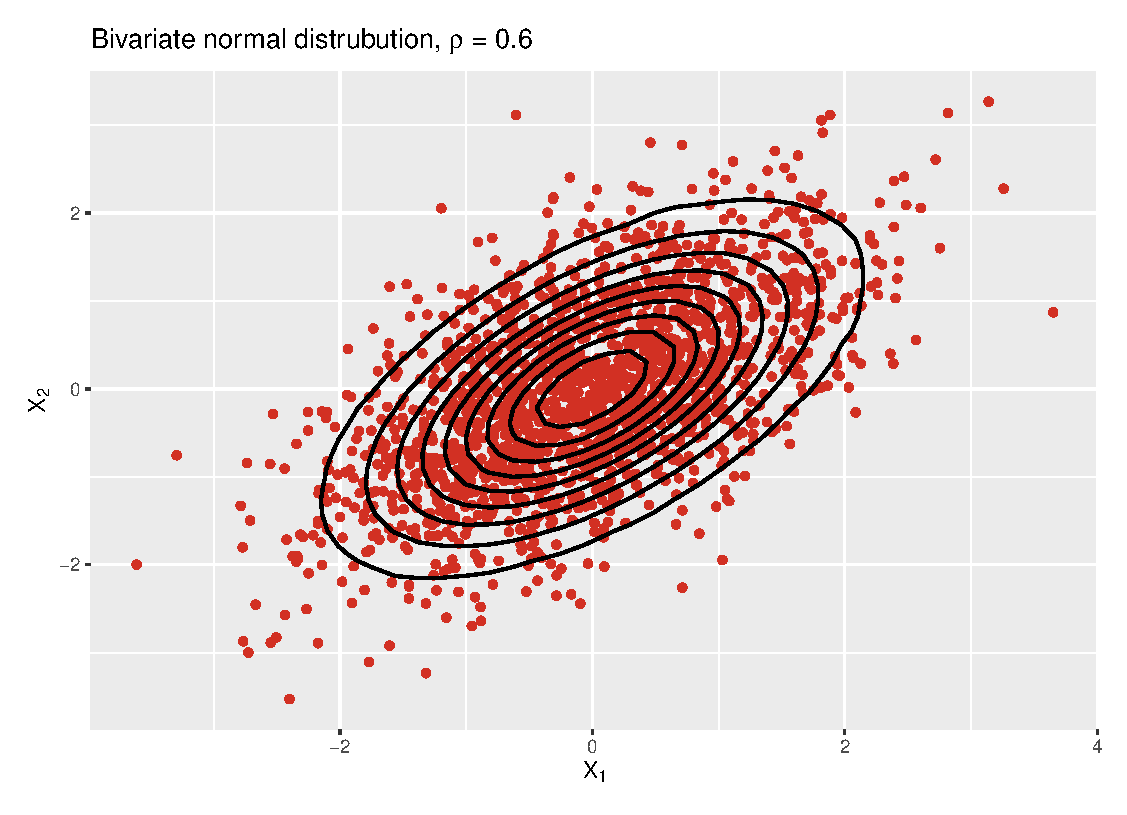
\includegraphics[width=\linewidth]{figures/bivariate_normal.eps}
  \caption{Gaussian distribution with contour lines}
  \label{fig:mvd_normal_copula}
\end{subfigure}
\begin{subfigure}{.45\textwidth}
  \centering
  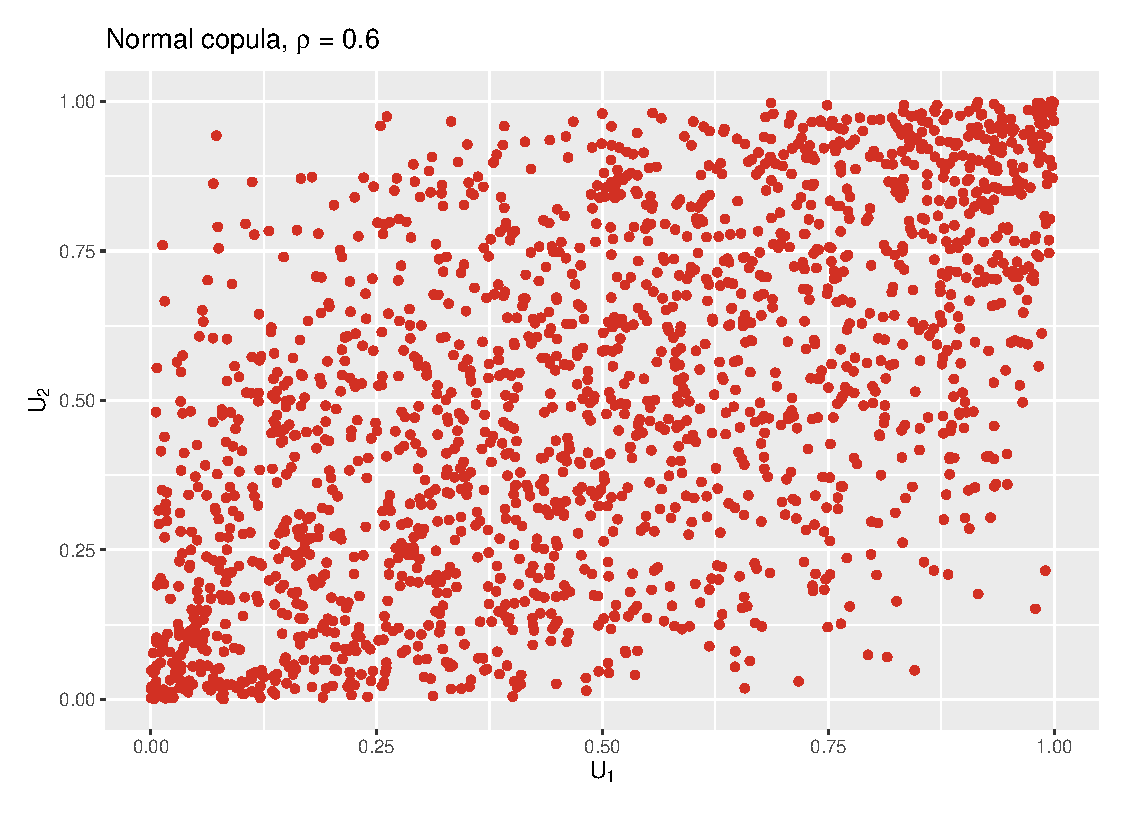
\includegraphics[width=\linewidth]{figures/normal_copula.eps}
  \caption{Gaussian copula}
  \label{fig:normal_copula}
\end{subfigure}
\caption{Bivariate Gaussian distribution and Gaussian copula for Pearson's $\rho = 0.6$ and simulated sample of size $n = 1800$, both with standard normal marginals}
\label{fig:normal_plots}
\end{figure}






\textbf{t-Copula}\\
Consider \ac{wlog} $\bm{X} \sim {t_{d}(\nu, \bm{0}, \mathbf{P})}$ (multivariate Student's t-distribution) with $\nu$ \ac{dof} and $\bm{P}$ a correlation matrix, then the \textit{t-copula (family)} is given by
\begin{equation}
C_{\nu, \bm{P}}^{t}(\mathbf{u})=t_{\nu, \bm{P}}\left(t_{\nu}^{-1}\left(u_{1}\right), \ldots, t_{\nu}^{-1}\left(u_{d}\right)\right),
\end{equation}
where $t_{\nu}$ is the \ac{CDF} of the univariate Student's t-distribution  and $t_{\nu, \bm{P}}$ is the \ac{CDF} of the multivariate Student's t-distribution (both with $\nu$ \ac{dof}).\\
For the \textit{bivariate t-copula} ($d=2$), the special cases are the same as for the Gaussian copula except that $d=0$ does not yield the independence copula (unless $\nu \rightarrow \infty$ in which case  $ C_{\nu, \rho}^{t} = C_{\rho}^{G a}$).\\
The density of $C_{\nu, \bm{P}}^{t}$ is given by
\begin{equation}
c_{\nu, \mathbf{P}}^{t}(\boldsymbol{u})=\frac{\Gamma((\nu+d) / 2)}{\Gamma(\nu / 2) \sqrt{\operatorname{det} \mathbf{P}}}\left(\frac{\Gamma(\nu / 2)}{\Gamma((\nu+1) / 2)}\right)^{d} \frac{\left(1+\boldsymbol{x}^{\prime} \mathbf{P}^{-1} \boldsymbol{x} / \nu\right)^{-(\nu+d) / 2}}{\prod_{j=1}^{d}\left(1+x_{j}^{2} / \nu\right)^{-(\nu+1) / 2}},
\end{equation}
where $\bm{x} = \left(t_{\nu}^{-1}\left(u_{1}\right), \ldots, t_{\nu}^{-1}\left(u_{d}\right)\right)$.

\hfill $\square$ \\






 \begin{figure}[H]
\centering
\begin{subfigure}{.45\textwidth}
  \centering
  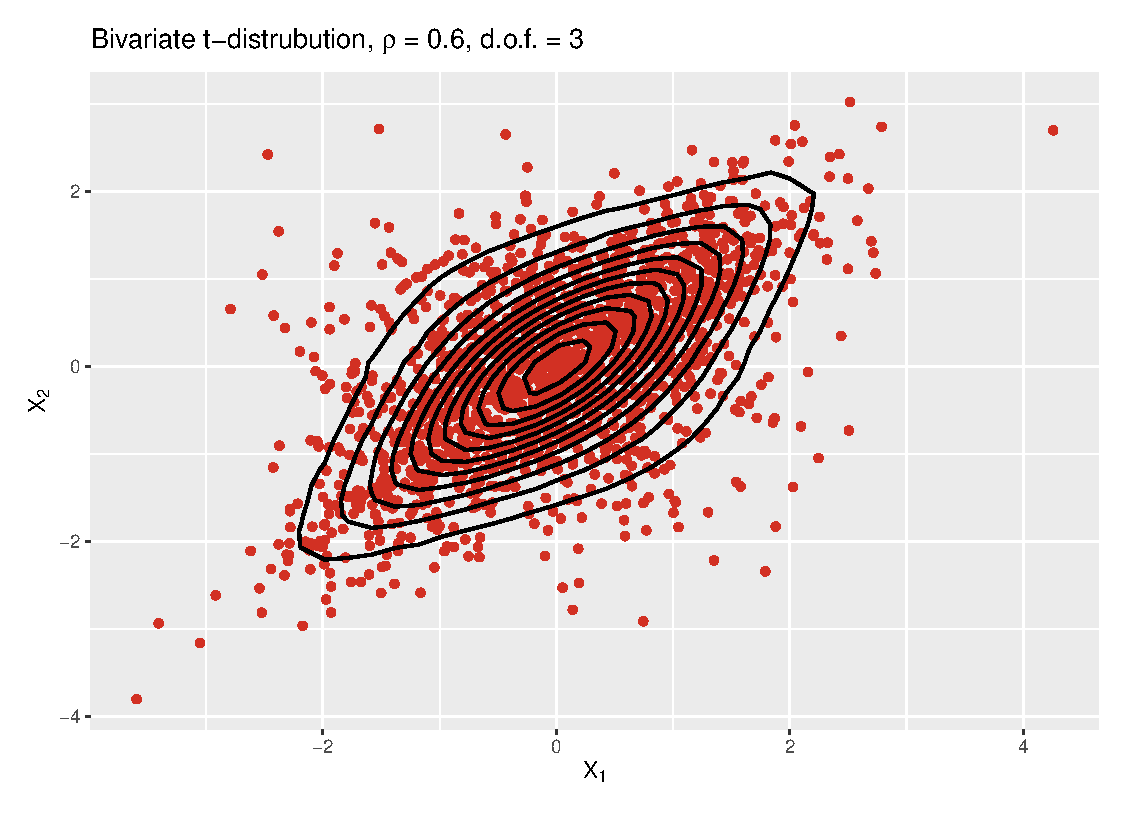
\includegraphics[width=\linewidth]{figures/bivariate_t.eps}
  \caption{t-distribution with contour lines}
  \label{fig:bivariate_t}
\end{subfigure}
\begin{subfigure}{.45\textwidth}
  \centering
  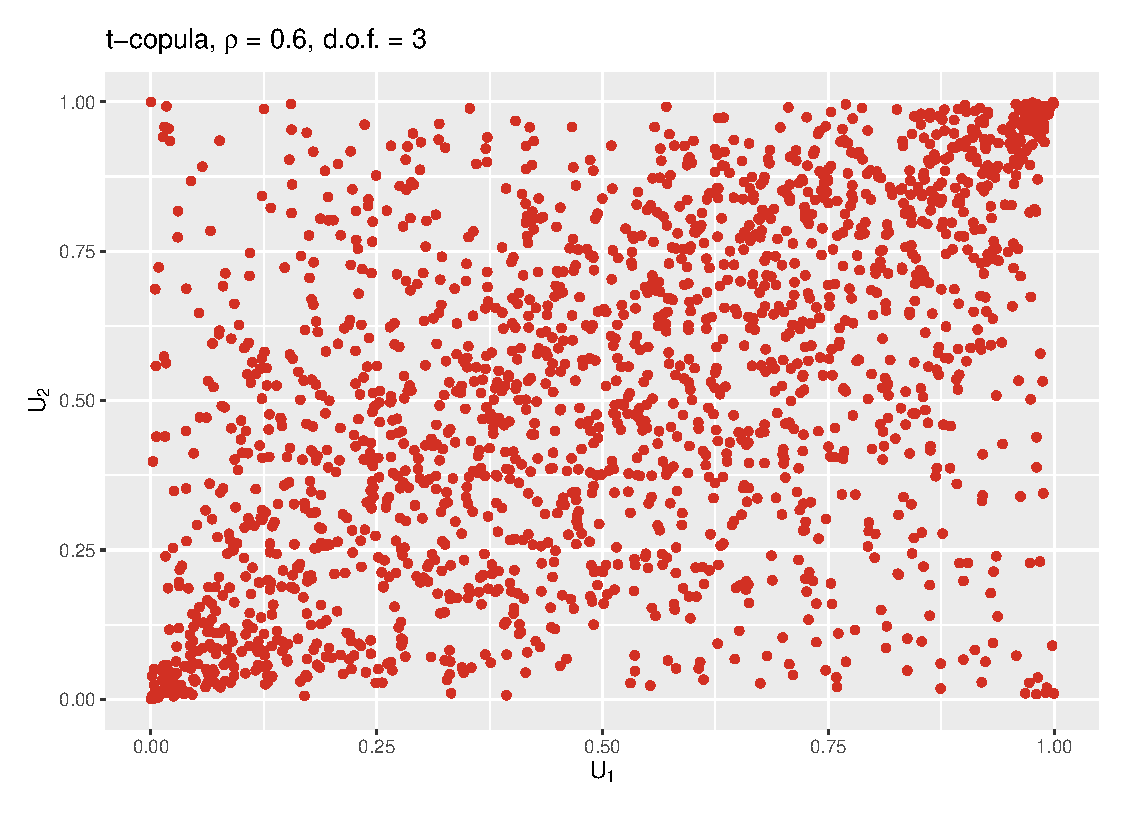
\includegraphics[width=\linewidth]{figures/t_copula.eps}
  \caption{t-copula}
  \label{fig:t_copula}
\end{subfigure}
\caption{Bivariate t-distribution and t-copula with 3 degrees of freedom for Pearson's $\rho = 0.6$ and simulated sample of size $n = 1800$, both with standard normal marginals}
\label{fig:t_plots}
\end{figure}






